\section{Sensorer}\label{sensorer}
Dette afsnit beskriver de forskellige sensorer der findes og som kunne være interessant for projektet. 

\paragraph{Kamera}
Kameraet kan tage billeder og billedesekvenser i form af video optagelse.

\paragraph{Accelerometer}
Accelerometeret måler accelerationen i x,y,z retningerne i et koordinatsystem der er lagt på telefonen som vist på \cref{analyse:accelerometer:koo}.
Accelerometret kan konceptuelt forstås som en kugle der ruller rundt i et rum hvor væggene kan måle den kraft de bliver påvirket med.
På \cref{analyse:accelerometer:kraft} ses dette konceptuelle rum med påvirkning fra tyngdekraften. 
Sensoren vil i dette tilfælde rapportere en negativ kraft i z-aksens retning.

\begin{figure}[h]
	\centering
	\begin{subfigure}[b]{0.47\textwidth}
		\centering
		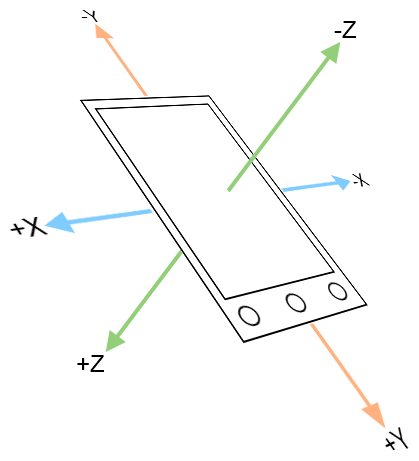
\includegraphics[width=.6\textwidth]{accelerometer-telefon}
		\caption{Koordinatsystem lagt på en telefon}
		\label{analyse:accelerometer:koo}
	\end{subfigure}
	~
	\begin{subfigure}[b]{0.47\textwidth}
		\centering
		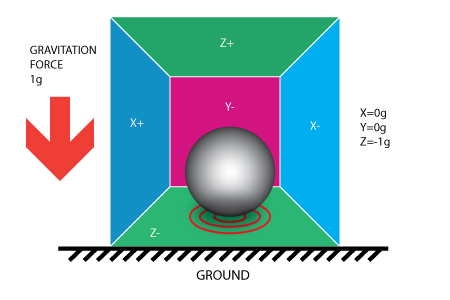
\includegraphics[width=\textwidth]{accelerometer}
		\caption{Konceptuel tegning af et accelerometers virkemåde. Illustration fra \cite{accelerometer}}
		\label{analyse:accelerometer:kraft}
	\end{subfigure}
	\caption{}
	\label{accelerometer}
\end{figure} 

\paragraph{GPS}
GPS sensoren giver en lokation som koordinater bestående af: breddegrad, længdegrad og en pejling.

\paragraph{Mikrofon}
Mikrofonen kan optage omgivelserne ved at konvertere akustisk lyd til elektriske signaler.

Lyd kan beskrives som bølger, der kan karakteriseres ved bølgens amplitude og frekvens.
Amplituden svarer til hvor høj en lyd opfattes og måles i decibel.
Frekvensen af en bølge bestemmer hvilken tone lyden er og måles i hertz. \cite{sound}


\paragraph{Lyssensor}
Lyssensoren kan måle belysningsstyrken på en flade i lux. Det er intensiteten af lyset der kan 'ses' på en flade. På \cref{fig:lux}  kan der ses eksempler.

\begin{figure}
	\centering
\begin{tabular}{ l | l}
	\textbf{Belysningsstyrke} & \textbf{Flader belyst af: }\\
\hline
0,27-1,0 lux &  Fuldmåne på en klar himmel \\
\hline
50 lux & Stue \\
\hline
80 lux & Kontor bygnings gang/toilet belysning \\
\hline
100 lux & Meget mørk overskyet dag \\
\hline
320-500 lux & Kontor belysning \\
\hline
400 lux & Solopgang eller solnedgang \\
\hline
1000 lux & Overskyet dag \\
\hline
10000-25000 lux & Fuld dagslys \\
\hline
32000-100000 lux & Direkte sollys\\
\hline
\end{tabular}
\caption{En tabel der viser belysningsstyrken på flader i lux under forskellige forhold. \citep{misc:lux}}
\label{fig:lux}
\end{figure}

\paragraph{Pulsmåler}
Pulsmåleren måler pulsen i hjerteslag per minut ved enten en elektrisk puls igennem et ledende materiale på huden, eller via en optisk sensor hvor man sætter fingeren på.
Den mest præcise måling fås hvis sensoren sidder spændt omkring brystet, mens sensorer der måler enten på håndleddet eller fingeren er mindre præcise \cite{burke1998precision}.

\paragraph{Galvanisk Hud Respons}
Galvanisk hud respons sensoren giver adgang til data omkring hvor god hud er til at lede strøm, huden leder strøm bedre jo mere den sveder, og derfor giver det også data omkring hvor meget den sveder.